% !TEX TS-program = pdflatex
% !TEX encoding = UTF-8 Unicode

% This file is a template using the "beamer" package to create slides for a talk or presentation
% - Talk at a conference/colloquium.
% - Talk length is about 20min.
% - Style is ornate.

% MODIFIED by Jonathan Kew, 2008-07-06
% The header comments and encoding in this file were modified for inclusion with TeXworks.
% The content is otherwise unchanged from the original distributed with the beamer package.

\documentclass{beamer}
%\usepackage{natbib}

% Copyright 2004 by Till Tantau <tantau@users.sourceforge.net>.
%
% In principle, this file can be redistributed and/or modified under
% the terms of the GNU Public License, version 2.
%
% However, this file is supposed to be a template to be modified
% for your own needs. For this reason, if you use this file as a
% template and not specifically distribute it as part of a another
% package/program, I grant the extra permission to freely copy and
% modify this file as you see fit and even to delete this copyright
% notice. 


\mode<presentation>
{
  \usetheme{Warsaw}
  % or ...

  \setbeamercovered{transparent}
  % or whatever (possibly just delete it)
}

\usepackage{tikz}
\usepackage{graphicx}
\usepackage[english]{babel}
% or whatever

\usepackage[utf8]{inputenc}
% or whatever

\usepackage{times}
\usepackage[T1]{fontenc}
% Or whatever. Note that the encoding and the font should match. If T1
% does not look nice, try deleting the line with the fontenc.


\title[Registrations and Pre-Analysis Plans] % (optional, use only with long paper titles)
{Registrations and Pre-Analysis Plans}

\subtitle
{Making research more transparent and reproducible}

\author[Author, Another] % (optional, use only with lots of authors)
{Garret Christensen\inst{1}}
% - Give the names in the same order as the appear in the paper.
% - Use the \inst{?} command only if the authors have different
%   affiliation.

\institute[Universities of Somewhere and Elsewhere] % (optional, but mostly needed)
{
  \inst{1}%
  Berkeley Initiative for Transparency in the Social Sciences\\
  University of California Berkeley\\
  and\\
  Center for Open Science
}
% - Use the \inst command only if there are several affiliations.
% - Keep it simple, no one is interested in your street address.

\date % (optional, should be abbreviation of conference name)
{BITSS Annual Meeting, 2014}
% - Either use conference name or its abbreviation.
% - Not really informative to the audience, more for people (including
%   yourself) who are reading the slides online

\subject{Research Transparency}
% This is only inserted into the PDF information catalog. Can be left
% out. 



% If you have a file called "university-logo-filename.xxx", where xxx
% is a graphic format that can be processed by latex or pdflatex,
% resp., then you can add a logo as follows:

% \pgfdeclareimage[height=0.5cm]{university-logo}{university-logo-filename}
% \logo{\pgfuseimage{university-logo}}



% Delete this, if you do not want the table of contents to pop up at
% the beginning of each subsection:
%\AtBeginSubsection[]
%{
%  \begin{frame}<beamer>{Outline}
%    \tableofcontents[currentsection,currentsubsection]
%  \end{frame}
%}


% If you wish to uncover everything in a step-wise fashion, uncomment
% the following command: 

\beamerdefaultoverlayspecification{<+->}


\begin{document}

\begin{frame}
  \titlepage
\end{frame}

\begin{frame}{Outline}
  \tableofcontents
  % You might wish to add the option [pausesections]
\end{frame}


% Structuring a talk is a difficult task and the following structure
% may not be suitable. Here are some rules that apply for this
% solution: 

% - Exactly two or three sections (other than the summary).
% - At *most* three subsections per section.
% - Talk about 30s to 2min per frame. So there should be between about
%   15 and 30 frames, all told.

% - A conference audience is likely to know very little of what you
%   are going to talk about. So *simplify*!
% - In a 20min talk, getting the main ideas across is hard
%   enough. Leave out details, even if it means being less precise than
%   you think necessary.
% - If you omit details that are vital to the proof/implementation,
%   just say so once. Everybody will be happy with that.

\section{Motivation}

\subsection{Publication Bias}
\begin{frame}{Publication Bias}%{Subtitles are optional.}
  % - A title should summarize the slide in an understandable fashion
  %   for anyone how does not follow everything on the slide itself.
  \begin{itemize}
  %\item
   %The distibution of published p-values jumps around .05 (Brodeur et al 2013).
  \item
  There is a higher fraction of rejected hypothesis tests in the social sciences than in physical sciences (Fanelli 2010).
  \item
  	Published null results are disappearing over time, in all disciplines (Fanelli 2011). 
  \item
    This is very unlikely to represent the true state of the universe.
  \item
  	Data on the complete set of experiments run shows strong results are 40pp more likely to be published, and 60pp more likely to be written up. The file drawer problem is massive. (Franco, Malhotra, Simonovits 2014---see tomorrow)
  \end{itemize}
\end{frame}

\begin {frame}{Publication Bias}
If we only write up/publish significant results, and we have no record of all the insignificant results, we have no way to tell if our `significant' results are real, or if they're the 5\% we should expect due to randomness.
\end{frame}

\subsection{P-Hacking}
\begin{frame}{P-Hacking}
\begin{itemize}
\pause
\item
Not something only evil people do. It can be subconcious.
\item
Also called fishing, researcher degrees of freedom, data mining, data massaging, or specification searching.
\item
Definition: flexibility in data analysis allows portrayal of \textit{anything} as below an arbitrary p-value threshhold; significance loses its meaning.
\end{itemize}
\end{frame}

{ % all template changes are local to this group.
    \setbeamertemplate{navigation symbols}{}
    \begin{frame}[plain]
    Does this 
    
    actually happen?
    
    (JLP 2011)
        \begin{tikzpicture}[remember picture,overlay]
            \node[at=(current page.center)] {
                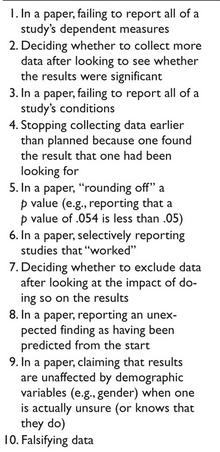
\includegraphics[height=\paperheight]{Prelec1.PNG}
            };
        \end{tikzpicture}
     \end{frame}
     
        
    \begin{frame}[plain]
         \begin{tikzpicture}[remember picture,overlay]
            \node[at=(current page.center)] {
                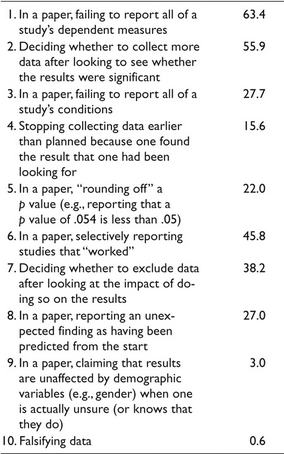
\includegraphics[height=\paperheight]{Prelec2.PNG}
            };
        \end{tikzpicture}
     \end{frame}
     
     \begin{frame}[plain]
         \begin{tikzpicture}[remember picture,overlay]
            \node[at=(current page.center)] {
                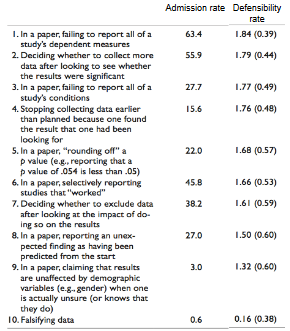
\includegraphics[height=\paperheight]{Prelec3.PNG}
            };
        \end{tikzpicture}
     \end{frame}
}
\begin{frame}{P-Hacking}
\begin{itemize}
\item
Do people actually do this? (Previous---John, Loewenstein, Prelec 2011)
\item
Listening to the Beatles' ``When I'm Sixty-Four'' makes you younger. (Simmons, Nelson, Simonsohn 2011)
\item
Inordinately many .049 p-values, and indordinately few .051's. (Brodeur et al 2013)
\item 
Political idiologues literally see in black and white (Nosek, Spies, Motyl 2012)
\end{itemize}
\end{frame}



\section{Solutions}
\subsection{Registration}
\begin{frame}{Solutions}
\begin{itemize}
\item
Publication Bias---Registration
\item
P-Hacking---Pre-Analysis Plans
\end{itemize}
\end{frame}

\begin{frame}{Registrations}
 \begin{itemize}
  \item
   Publicly stating all research you do, what hypotheses you test, prospectively.
   %\item If we know every hypothesis test that is run on a given subject, we have a better idea of how seriously to take the significant results.
  \item
   Near universal adoption in medical RCTs. \url{http://clinicaltrials.gov}
   \item Newer to social sciences, but:
   \begin{itemize}
   \item
   	AEA registry \url{http://socialscienceregistry.org}
   \item
    EGAP registry \url{http://egap.org/design-registration}
   \item 
    3ie registry \url{http://ridie.3ieimpact.org}
   \item
   	Open Science Framework \url{http://osf.io}
   	\begin{itemize}
   	\item
   	Open format
   	\item
   	Will soon sync with above
   	\end{itemize}
   \end{itemize}
  \end{itemize}  
\end{frame}


\subsection{Pre-Analysis Plan}
\begin{frame}{Pre-Analysis Plan}
\pause
\begin{itemize}
\item
Often part of a registration
\item
From 3ie: ``A pre-analysis plan is a detailed description of the analysis to be conducted that is written in advance of seeing the data on impacts of the program being evaluated. It may specify hypotheses to be tested, variable construction, equations to be estimated, controls to be used, and other aspects of the analysis. A key function of the pre-analysis plan is to increase transparency in the research. By setting out the details in advance of what will be done and before knowing the results, the plan guards against data mining and specification searching. Researchers are encouraged to develop and upload such a plan with their study registration, but it is not required for registration.''
\end{itemize}
\end{frame}

\begin{frame}{Glennerster, Takavarasha Suggestions}
\pause
\begin{enumerate}
\def\labelenumi{\arabic{enumi}.}
\item
  the main outcome measures,
\item
  which outcome measures are primary and which are secondary,
\item
  the precise composition of any families that will be used for mean
  effects analysis,
\item
  the subgroups that will be analyzed,
\item
  the direction of expected impact if we want to use a one-sided test,
  and
\item
  the primary specification to be used for the analysis.
\end{enumerate}
\end{frame}

\begin{frame}{McKenzie Suggestions}
\pause
\url{http://blogs.worldbank.org/impactevaluations/a-pre-analysis-plan-checklist}

\begin{enumerate}
\item
  Description of the sample to be used in the study
\item
  Key data sources
\item
  Hypotheses to be tested throughout the causal chain
\item
  Specify how variables will be constructed
\item
  Specify the treatment effect equation to be estimated
\item
  What is the plan for how to deal with multiple outcomes and multiple
  hypothesis testing?
\item
  Procedures to be used for addressing survey attrition
\item
  How will the study deal with outcomes with limited variation?
\item
  If you are going to be testing a model, include the model
\item
  Remember to archive it
\end{enumerate}
\end{frame}

\begin{frame}{Simmons, Nelson, Simonsohn (2011)}
\pause
\begin{enumerate}
\def\labelenumi{\arabic{enumi}.}
\item
  Authors must decide the rule for terminating data collection before
  data collection begins and report this rule in the article.
\item
  Authors must collect at least 20 observations per cell or else provide
  a compelling cost-of-data-collection justification.
\item
  Authors must list all variables collected in a study.
\item
  Authors must report all experimental conditions, including failed
  manipulations.
\item
  If observations are eliminated, authors must also report what the
  statistical results are if those observations are included.
\item
  If an analysis includes a covariate, authors must report the
  statistical results of the analysis without the covariate.
\end{enumerate}

\end{frame}

\begin{frame}{Examples}
J-PAL Hypothesis Registry (9)

\end{frame}
%\section{Implementation}
%\begin{frame}{AEA Trial Registration}
%\end{frame} 
%\begin{frame}{EGAP Registration}
%\end{frame}
%\begin{frame}{3ie Registration}
%\end{frame}
%\begin{frame}{Open Science Framework}
%\end{frame}

\section{Conclusion}
\begin{frame}{Conclusion}
 \begin{itemize}
 \item
  Not just for RCTs. 
 \item
  Spectrum from confirmatory to exploratory research, all has value.
 \item
  I'd just like know which research is which.
\end{itemize}

\end{frame}

%\begin{frame}{References}
%\bibliographystyle{plainnat}
%\bibliography{Bibliography}
%\end{frame}
%%%%%%%%%%%%%%%%%%%%%%%%%%%%%%%%%%%%%%%%%%%5
\iffalse
%\begin{frame}{P-Hacking}
%  You can create overlays\dots
%  \begin{itemize}
%  \item using the \texttt{pause} command:
%    \begin{itemize}
    \item
      First item.
      \pause
    \item    
      Second item.
    \end{itemize}
  \item
    using overlay specifications:
    \begin{itemize}
    \item<3->
      First item.
    \item<4->
      Second item.
    \end{itemize}
  \item
    using the general \texttt{uncover} command:
    \begin{itemize}
      \uncover<5->{\item
        First item.}
      \uncover<6->{\item
        Second item.}
    \end{itemize}
  \end{itemize}
\end{frame}


\subsection{Previous Work}

\begin{frame}{Make Titles Informative.}
\end{frame}

\begin{frame}{Make Titles Informative.}
\end{frame}



\section{Our Results/Contribution}

\subsection{Main Results}

\begin{frame}{Make Titles Informative.}
\end{frame}

\begin{frame}{Make Titles Informative.}
\end{frame}

\begin{frame}{Make Titles Informative.}
\end{frame}


\subsection{Basic Ideas for Proofs/Implementation}

\begin{frame}{Make Titles Informative.}
\end{frame}

\begin{frame}{Make Titles Informative.}
\end{frame}

\begin{frame}{Make Titles Informative.}
\end{frame}



\section*{Summary}

\begin{frame}{Summary}

  % Keep the summary *very short*.
  \begin{itemize}
  \item
    The \alert{first main message} of your talk in one or two lines.
  \item
    The \alert{second main message} of your talk in one or two lines.
  \item
    Perhaps a \alert{third message}, but not more than that.
  \end{itemize}
  
  % The following outlook is optional.
  \vskip0pt plus.5fill
  \begin{itemize}
  \item
    Outlook
    \begin{itemize}
    \item
      Something you haven't solved.
    \item
      Something else you haven't solved.
    \end{itemize}
  \end{itemize}
\end{frame}



% All of the following is optional and typically not needed. 
\appendix
\section<presentation>*{\appendixname}
\subsection<presentation>*{For Further Reading}

\begin{frame}[allowframebreaks]
  \frametitle<presentation>{For Further Reading}
    
  \begin{thebibliography}{10}
    
  \beamertemplatebookbibitems
  % Start with overview books.

  \bibitem{Author1990}
    A.~Author.
    \newblock {\em Handbook of Everything}.
    \newblock Some Press, 1990.
 
    
  \beamertemplatearticlebibitems
  % Followed by interesting articles. Keep the list short. 

  \bibitem{Someone2000}
    S.~Someone.
    \newblock On this and that.
    \newblock {\em Journal of This and That}, 2(1):50--100,
    2000.
  \end{thebibliography}
\end{frame}
\fi


\end{document}


